\documentclass[english,11pt,a4paper]{article}
\usepackage[utf8]{inputenc}
\usepackage{mathtools}	%
\usepackage{amssymb} % Mathematik und Dinge wie \qquad
\usepackage[T1]{fontenc} %Anführungszeichen
\usepackage{graphicx} %Bilder
\graphicspath{/Users/Nata/Documents/Master/M Prak Biophysics/Genetic Toogle Switch}
\usepackage{subcaption} %figures nebeneinander
\usepackage[labelformat=simple]{caption} %Bildunterschriften
\usepackage{setspace}
\usepackage{nicefrac}
\usepackage{longtable}
\usepackage[english]{babel}
\usepackage{array}
\usepackage{float}
\usepackage{geometry}
\usepackage{physics}
\usepackage[colorlinks=false]{hyperref}
\usepackage[miktex, subfolder]{gnuplottex}
%\usepackage[parfill]{parskip} % Absätze nicht eingerückt sondern durch Leere Zeilen getrennt
\setlength\parindent{0pt}
%
\usepackage{biblatex}
\usepackage{filecontents}
\usepackage{bibgerm}
\usepackage{url}

\usepackage{chemmacros,upgreek} 
\NewChemParticle\neutrino{\chemnu_{$\!e$}} 
\NewChemParticle\antineutrino{$\bar{\chemnu}$_{$\!e$}} 

\NewChemParticle\betaminus{\chembeta-} 
\NewChemParticle\betaplus{\chembeta+}


\begin{filecontents}{quellen.bib}	
{
	@online{1,
		title = {Manual},
		url = {http://apcmbp.uni-koeln.de/sites/biophyspraktikum/Prelab_Manual_FRET.pdf},
		urldate = {2017-12-02},
	}
	@online{2,
		title = {Refractive index of water},
		url = {http://hyperphysics.phy-astr.gsu.edu/hbase/Tables/indrf.html},
		urldate = {2017-12-02},
	}
	@online{3,
		title = {Quantum yield of Cy3},
		url = {http://www.atdbio.com/content/32/Cyanine-dyes},
		urldate = {2017-12-02},
	}
	@online{4,
		title = {Extinction coefficient of Cy5},
		url = {http://www.sigmaaldrich.com/technical-documents/protocols/biology/sample-labeling-and-processing.html},
		urldate = {2017-12-02},
	}
	@online{5,
		title = {Fluorescence spectroscopy},
		url = {https://de.wikipedia.org/wiki/Fluoreszenzspektroskopie},
		urldate = {2017-12-02},
	}

	@online{6,
		title = {Förster Radius of Cy3-Cy5},
		url = {https://web.stanford.edu/class/cs379c/archive/2013/class_messages_listing/figures/fluorescence_resonance_energy_transfer.pdf},
		urldate = {2018-01-12},
	}
}
\end{filecontents}
\addbibresource{quellen.bib}

\linespread{1.4}

%================================================================================

\begin{document}

\begin{titlepage}
	\centering
	\huge
	\textbf{Genetic toggle switch}
	
	\vspace{1cm}
	\huge
	Advanced Practical course in Biophysics
	
	\vspace{0.8cm}
	\normalsize
	At the
	
	\vspace{0.5cm}
	\Large
	Institute for Theoretical Physics, Cologne
	
	\vspace{1cm}
	\normalsize
	Submitted on 2.12.2017
	
	\vspace{1.5cm}
	\begin{figure}[h]
		\centering
	%	\includegraphics[width=150pt]{resources/uni_logo.png}
	\end{figure}
	
	\vspace{2.5cm}
	\small
	
	\begin{centering}
		\begin{tabular}{lll}
			& \textbf{Students} & \hspace{5cm} \textbf{Instructor} \\
			& Simon Barton 5963508 & \hspace{5cm} Martin Lukacisin \\
			& Galib Hassan 6057349\\
			& Natawan Gadjisade 6045910
		\end{tabular}
	\end{centering}
	
\end{titlepage}

\pagenumbering{Roman}  
\tableofcontents

\pagebreak
\pagenumbering{arabic}

\addcontentsline{toc}{section}{Introduction}
\section*{Introduction}

A genetic toggle switch has a similar function as a flip flop in electronics.
In a genetic circuits the genetic toggle switch can exhibits two stable steady states and store 1 bit of information.
In this experiment we are observing the behaviour of a genetic toggle switch as well as its switching between two stable states (two different fluorescent proteins with different colours, green and red) bacteria E.Coli is observed..
As the E.coli bacteria are genetic modified with two different promoters which not only control the expression of two genes but also the expression of a repressor for each other, the system is in a steady state of the circuit.   
Measuring the fluorescence of the system allows us  to determine the concentration of the inducer that is needed to cause a switching between the green and red fluorescent protein.

\newpage
\part{Theoretical background}

\section{Synthetically controlling gene expression}

The idea behind synthetic gene regularity circuits such as toggle switch is that the transcription of the gene is controlled by inducible promoters by changing the external concentration of an inducer.
It is a easy way to turn genes on and off and to control their level of expression.
The most used inducible promoters are the lac promoter and the tet promoter. 
The transcription factors (such as lac repressor lacl and the tet repressor TetR, respectively) bind to the promoter and repress the transcription of the promoter. 
These repressors can bind to specific inducers as IPTG or aTc. 
The change in protein conformation followed from a change in affinity for the binding site in the promoter region is achieved by the binding of the inducers to the repressors.
The advantage of IPTG and aTc is that they do not have other effect on the cell beside of changing the binding affinity of the respective repressors.

In this experiment the inducible promoters control a reporter gene (e.g fluorescent protein such GFP) and are put on the chromosome or on a plasmid inside a bacterium like E.Coli. 
In growth medium these bacteria are then cultured that can be supplemented with the respective inducer.

\begin{figure}[htbp] 
  \centering
     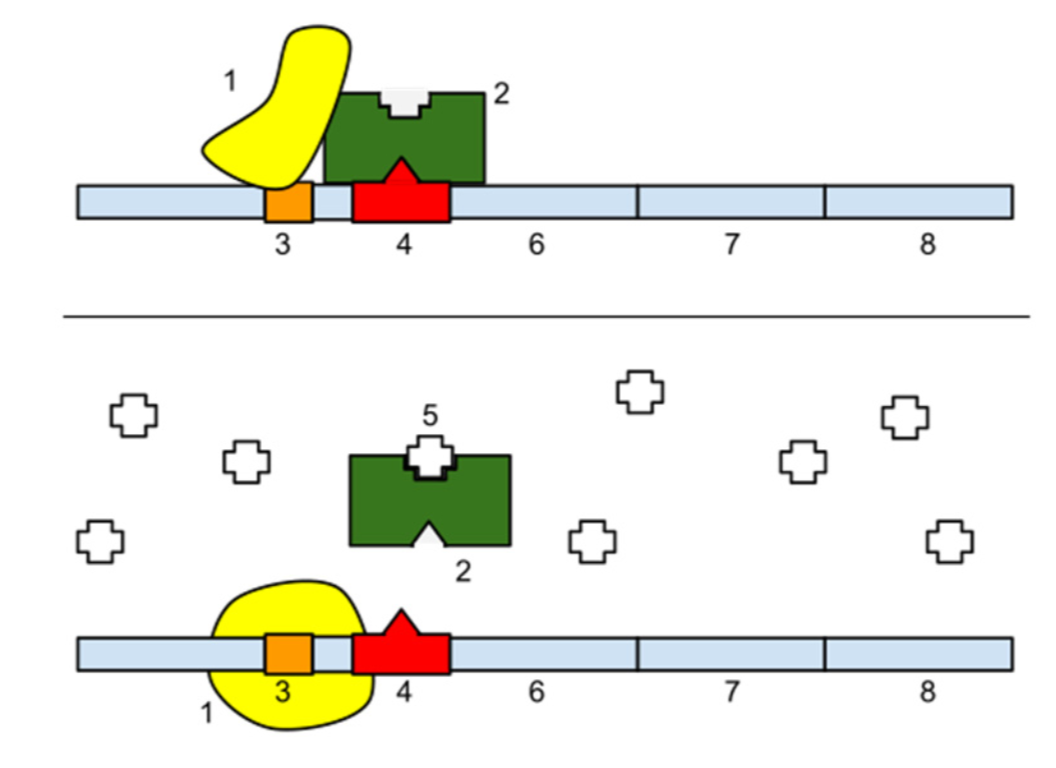
\includegraphics[width=0.7\textwidth]{IPTG}
  \caption{Inducible control of the lac promoter using IPTG. 1: RNA polymerase, 2:Repressor, 3:Promoter, Operator, 5: Lactose, 6-8: lac operon or other genes under the control of the lac promotor. 
 First scheme: The promoter is turned off. No lactose or IPTG is there to block the lac repressor, so the repressor and promoter are tightly bound to the operator, which obstructs the RNA polymerase from binding to the promoter.
Second scheme: The promoter is turned on. Lactose inhibits the repressor, allowing RNA polymerase to bind the promoter and express the downstream genes. Source: Manual of practical course. }
  \label{fig:Bild1}
\end{figure}



\newpage

\section{Design of toggle switch circuit} 

The goal is to obtain two district states of gene expression that are stable over a long. 
This construction consists of two promoters. Each is controlling the the expression of the repressor of the other promoter. 
It allows us to have to possible states. (a) Promoter 2 is shut down as promoter 1 is highly expressed, which leads to many copies of repressor 2.
(b) Promoter 1 is shut down as the promoter 2 is highly expressed, which leads to many copies of repressor 1.

More precisely, here the lac promoter (repressed by Lacl) controls the expression of tetR while the tet promoter (repressed by TetR) controls the expression of lacl. Also the expression of a gfp gene and an mcherry gene is controlled from tet promoter and lac promoter, respectively. 
It is possible to read out the state of the system by measuring fluorescence as gfp code for green and mcherry for red fluorescent proteins (GFP and RFP).
Adding the inducers IPTG or aTc leads to a flipping of the system.


\begin{figure}[htbp] 
  \centering
     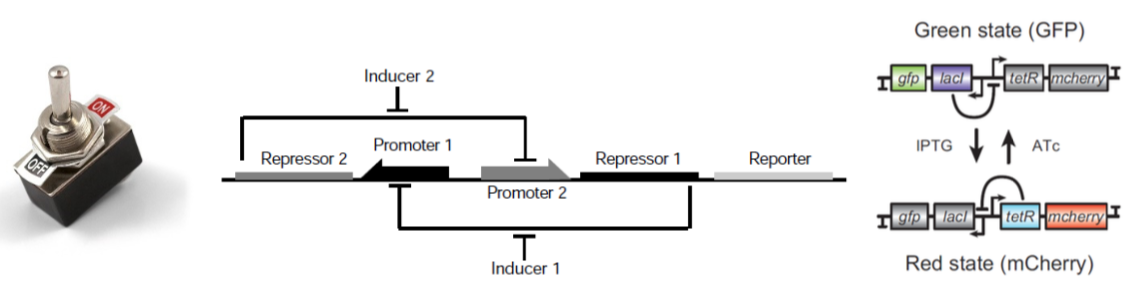
\includegraphics[width=0.9\textwidth]{Design}
  \caption{ Genetic toggle switch. First: electrical toggle switch with a mechanical lever. Second: General design of a genetic toggle switch. Third: Specific circuit used in this experiment (Lee et al.2016). IPTG and aTc can be used to flip the toggle switch from the green to the red state and vice versa, respectively. Source: Manual of practical course }
  \label{fig:Bild2}
\end{figure}

\newpage
\section{Experimental techniques and procedure}

We want to determine the average state of the synthetic toggle switch circuit in a population of cells. For that we have to measure the intracellular concentration of the green and the red fluorescent protein. 
The simplest way is to measure the total fluorescence intensity and normalising it to the total biomass of the population. 
We are using an \textbf{optical density (OD)} measurement to get the biomass of a growing bacterial culture as it is approximately equal to the total cell volume.
The absorbance is measured in a spectrophotometer according to Beer-Lambert law, which is proportional to the biomass density of the culture. Furthermore, measuring the optical density over time allows to determine the specific growth rate.
\\
The individual cells should be after switching either in one of two distinct gene expression states. Here: green or red. 
To observe the single-cell fluorescence we are using a \textbf{fluorescence microscopy} where individual cells are directly visualised.
\bigskip

In our experiment we had two overnight cultures one in green state and another in red state. The first step was to set up an IPTG and an aTc concentration gradient in glucose M9 medium with chloramphenicol. After that we had to inoculate the wells containing the IPT concentration gradient in the green state and the wells containing aTc from the overnight culture in the red state, ending up with the same ratio of volume of medium containing inducer to volume of overnight culture.
We took measurement of the optical density from the GFP and RFP fluorescence every $\approx$ 30min. and simultaneously pictures with the microscope of the overnight cultures.Furthermore, pictures of the GRP and RFP overnight cultures including IPTG and aTc, respectively in the highest concentration were taken.


 \newpage
\part{Results}

\section{Discussion}


\pagebreak

\addcontentsline{toc}{section}{References}
\printbibliography

\end{document}







































